\section{pk2cmd}
\label{sec:pk2cmd}
Das pk2cmd Commandline-Tool ermöglicht Linux (Es gibt auch eine Mac und Windows Version) mit dem PICkkit 2 PIC-Microchip über den Terminal anzusteuern. Hier wird es dafür benötigt um den compilierten Assembler-Code auf den PIC-Microchip zu laden.

\subsection{Installation}
\label{sub:installation}
Quelle: \url{https://www.making-sound.co.uk/tech-notes/pickit2-linux.html}\\

\begin{itemize}
    \item[1)] Zuerst ladet man die nötigen Pakete um pk2cmd zu installieren. Das erfolgt über diesen Befehl im Terminal:
    \begin{lstlisting}[language=bash]
    sudo apt install build-essential libusb-dev
    \end{lstlisting}
    \item[2)] Lade \href{https://github.com/psmay/pk2cmd}{pk2cmd von GitHub} und entpacke Sie den Download in Ihrem Download Ordner. Öffnen Sie dann den Terminal und navigieren zum diesem Ordner-Verzeichnis.
    \begin{lstlisting}
    cd ~/Downloads/pk2cmd/pk2cmd
    \end{lstlisting}
    
    Alternative mit git über Terminal herunterladen und in das Verzeichnis navigieren:
    \begin{lstlisting}
    git clone https://github.com/psmay/pk2cmd.git
    cd pk2cmd/pk2cmd
    \end{lstlisting}
    \item[3)] Zum installieren führen Sie folgende Befehle aus:
    \begin{lstlisting}[language=bash]
    make linux
    \end{lstlisting}
    \item[4)] Zum Testen von pk2cmd führen Sie diesen Command im selben Ordner aus:
    \begin{lstlisting}[language=bash]
    sudo ./pk2cmd -?V -B./
    \end{lstlisting}
    \begin{center}
        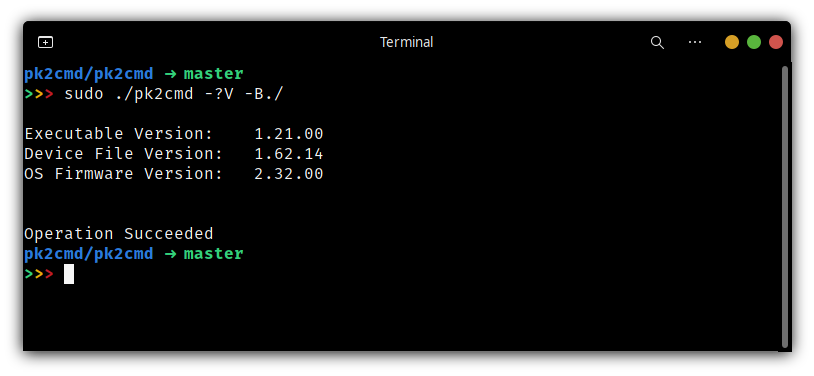
\includegraphics[scale = 0.5]{pk2cmd_test.png}
    \end{center}
    \newpage
    \item[5)] Zum Testen ob der PIC-Microchip von pk2cmd angesteuert wird kann dieser Command im selben Ordner ausgeführt werden:
    \begin{lstlisting}[language=bash]
    sudo ./pk2cmd -B./ -I -P
    \end{lstlisting}
    \begin{center}
        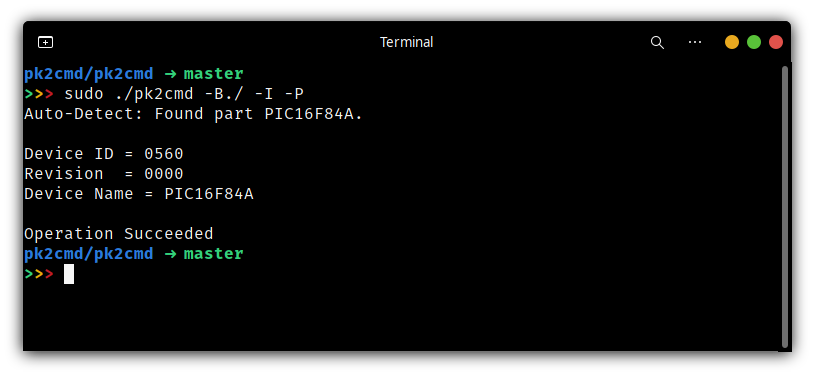
\includegraphics[scale = 0.5]{pk2cmd_test_PIC.png}
    \end{center}
    \item[6)] Nun wird der Command \enquote{pk2cmd} global zugänglich gemach mit diesem Befehl, welcher wieder im selben Ordner ausgeführt werden muss:
    \begin{lstlisting}[language=bash]
    echo 'export PATH="$PATH:/usr/share/pk2"' >> ~/.bashrc
    \end{lstlisting}
    Danach kann man den Ordner verlassen und den globalen Befehl wie folgt testen:
    \begin{lstlisting}[language=bash]
    cd
    pk2cmd -?V
    \end{lstlisting}
    \begin{center}
       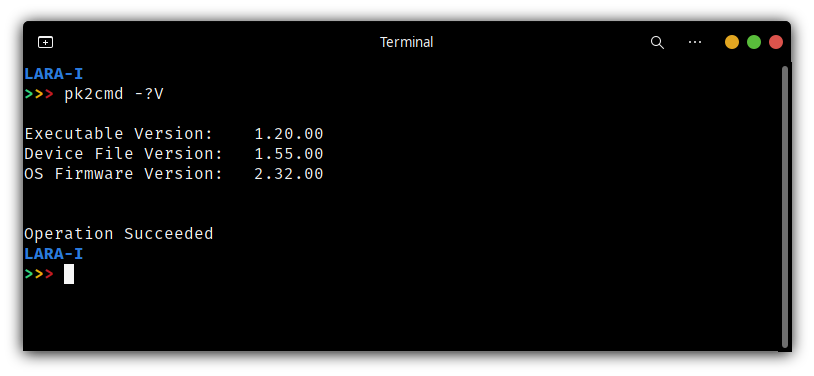
\includegraphics[scale = 0.5]{pk2cmd_test_global.png}
    \end{center}
\end{itemize}
Bei Problemen ist in der Quelle ein Troubleshooting aufgeführt, welches Ihnen bestimmt weiter helfen wird. Dies wird aber hier bewusst weggelassen, da ab nun alles funktionieren sollte.
\newpage
\subsection{Befehlspalette}
\label{sub:commands}
Quelle: \url{https://github.com/kvadevack/pk2cmd/blob/master/pk2cmd/release/Readme%20For%20PK2CMD.txt}
\begin{center}
\begin{lstlisting}[language=bash]
PICkit 2 COMMAND LINE HELP
Options              Description                              Default
-----------------------------------------------------------------------------
A<value>             Set Vdd voltage                          Device Specific
B<path>              Specify the path to PK2DeviceFile.dat    Searches PATH
                                                              and calling dir
C                    Blank Check Device                       No Blank Check
D<file>              OS Download                              None
E                    Erase Flash Device                       Do Not Erase
F<file>              Hex File Selection                       None
G<Type><range/path>  Read functions                           None
                     Type F: = read into hex file,
                             path = full file path,
                             range is not used
                     Types P,E,I,C: = ouput read of Program,
                             EEPROM, ID and/or Configuration
                             Memory to the screen. P and E
                             must be followed by an address
                             range in the form of x-y where
                             x is the start address and y is
                             the end address both in hex,
                             path is not used
                             (Serial EEPROM memory is 'P')
H<value>             Delay before Exit                        Exit immediately
                         K = Wait on keypress before exit
                         1 to 9 = Wait <value> seconds
                                  before exit
I                    Display Device ID & silicon revision     Do Not Display
J<newlines>          Display operation percent complete       Rotating slash
                         N = Each update on newline
K                    Display Hex File Checksum                Do Not Display
L<rate>              Set programming speed                    Fastest
                     <rate> is a value of 1-16, with 1 being
                     the fastest.

M<memory region>     Program Device                           Do Not Program
                     memory regions:
                         P = Program memory
                         E = EEPROM
                         I = ID memory
                         C = Configuration memory
                         If no region is entered, the entire
                         device will be erased & programmed.
                         If a region is entered, no erase
                         is performed and only the given 
                         region is programmed.
                         All programmed regions are verified.
             (serial EEPROM memory is 'P')
N<string>            Assign Unit ID string to first found     None
                     PICkit 2 unit.  String is limited to 14
                     characters maximum.  May not be used
                     with other options.
                     Example: -NLab1B
P<part>              Part Selection. Example: -PPIC16f887     (Required)
P                    Auto-Detect in all detectable families
PF                   List auto-detectable part families
PF<id>               Auto-Detect only within the given part
                     family, using the ID listed with -PF
                     Example: -PF2
Q                    Disable PE for PIC24/dsPIC33 devices     Use PE
R                    Release /MCLR after operations           Assert /MCLR
S<string/#>          Use the PICkit 2 with the given Unit ID  First found unit
                     string.  Useful when multiple PICkit 2
                     units are connected.
                     Example: -SLab1B
                     If no <string> is entered, then the
                     Unit IDs of all connected units will be
                     displayed.  In this case, all other
                     options are ignored. -S# will list units
                     with their firmware versions.
                     See help -s? for more info.
T                    Power Target after operations            Vdd off
U<value>             Program OSCCAL memory, where:            Do Not Program
                      <value> is a hexidecimal number
                      representing the OSCCAL value to be
                      programmed. This may only be used in
                      conjunction with a programming 
                      operation.
V<value>             Vpp override                             Device Specific
W                    Externally power target                  Power from Pk2
X                    Use VPP first Program Entry Method       VDD first
Y<memory region>     Verify Device                            Do Not Verify
                         P = Program memory
                         E = EEPROM
                         I = ID memory
                         C = Configuration memory
                         If no region is entered, the entire
                         device will be verified.
                         (Serial EEPROM memory is 'P')
Z                    Preserve EEData on Program               Do Not Preserve
?                    Help Screen                              Not Shown









     Each option must be immediately preceeded by a switch, Which can
     be either a dash <-> or a slash </> and options must be separated
     by a single space.

     Example:   PK2CMD /PPIC16F887 /Fc:\mycode /M
                               or
                PK2CMD -PPIC16F887 -Fc:\mycode -M

     Any option immediately followed by a question mark will invoke
     a more detailed description of how to use that option.

     Commands and their parameters are not case sensitive. Commands will
     be processed according to command order of precedence, not the order
     in which they appear on the command line. 
    Precedence:
                -?      (first)
                -B
        -S
                -D	
        -N
                -P
                -A -F -J -L -Q -V -W -X -Z
                -C
                -U
                -E
                -M
                -Y
                -G
                -I -K   
        -R -T
        -H      (last)
        
     The program will return an exit code upon completion which will
     indicate either successful completion, or describe the reason for
     failure. To view the list of exit codes and their descriptions,
     type -?E on the command line.

     type -?V on the command line for version information.

     type -?L on the command line for license information.

     type -?P on the command line for a listing of supported devices.
     type -?P<string> to search for and display a list of supported devices
                      beginning with <string>.

---------------------------------------------------------------------------
\end{lstlisting}
\end{center}
\newpage
\subsection{Verwendung}
\label{sub:howToUse}
Um nun ein gegebenes {\ttfamily foo.hex}-File auf einen PIC-Microchip in unseren Fall der PIC16F84A zu laden wird folgender Befehl im Terminal ausgeführt:
\begin{lstlisting}[language=bash]
                pk2cmd -A5 -PPIC16F84A -F foo.hex -M -T -R
\end{lstlisting}
Nach dem ausüben dieses Befehls sollte der Microchip das Programm ausführen. Was die jeweiligen Attribute des Befehls festlegen, kann im Kapitel \ref{sub:commands} nachgelesen werden.